\input{../../.preambles/01-semester_work}
\input{../../.preambles/10-russian}
\input{../../.preambles/20-math}
\input{../../.preambles/30-physics}
\usepackage{wrapfig}

\begin{document}
\maketitlepage{Факультет электроники и вычислительной техники}{физики}
{Вакуумная и газоразрядная электроника}{}{18}{студент группы Ф-369\\Голубев~А.~В.}
{}{доцент Ковтун~Д.~Г.}{}{}

\emph{Задача №1:} Электрон со скоростью \( v \) влетает в область, где 
существуют коллинеарные однородные электрическое \( E \) и магнитное \( B \) 
поля, под углом \( \alpha \) к направлению полей. Определить траекторию 
его движения и время, за которое он достигнет экрана, находящегося на 
расстоянии \( L \) от плоскости влёта, и координаты точки на экране.

\emph{Решение:}

\begin{wrapfigure}[8]{l}{0.5\textwidth}
    \vspace{-2ex}
    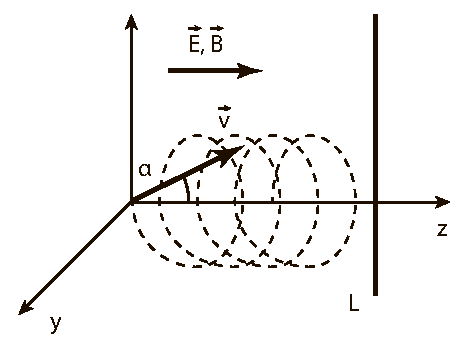
\includegraphics[width=0.5\textwidth]{images/im_01}
\end{wrapfigure}

Запишем силу действующую на электрон со стороны полей:
\[
	m\vec{a} = q\left( \vec{E} + \vec{v}\times\vec{B} \right)
\]
\[
	\vec{v}\times\vec{B} = 
	\begin{vmatrix}
		\vec{e_x} & \vec{e_y} & \vec{e_z} \\
		\dot{x}   & \dot{y}   & \dot{z}   \\
		0         & 0         & B
	\end{vmatrix}
\]

Расписывая определитель получаем систему уравнений:
\[
	\left\{ \begin{array}{ll}
		m\ddot{x} = q\dot{y}B \\
		m\ddot{y} = -q\dot{x}B \\
		m\ddot{z} = qE
	\end{array} \right.
	\quad
	\left\{ \begin{array}{ll}
		\ddot{x} = \omega_c\dot{y} \\
		\ddot{y} = -\omega_c\dot{x} \\
		\ddot{z} = \cfrac{q}{m}E
	\end{array} \right.
\]
где обозначим за \( \omega_c = \cfrac{q}{m}B \)

Найдём время за которое электрон достигнет экрана. Из уравнения 
\[ \ddot{z} = \cfrac{q}{m}E \]

Проинтегрировав уравнение по времени получим:
\[
	z = \frac{q}{2m}Et^2 + v_{z0}t
\]

Подставляя расстояние \( L \) до экрана найдём время:
\[
	L = \frac{q}{2m}Et^2 + v_{z0}t \quad\Rightarrow\quad
	\frac{q}{2m}Et^2 + v_{z0}t - L = 0
\]
\[
	t^2 + \frac{2mv_{z0}}{qE}t - \frac{2mL}{qE} = 0
\]
\[
	t = -\cfrac{mv_{z0}}{qE} + 
	\sqrt{ \cfrac{m}{qE}\left( \cfrac{mv^2_{z0}}{qE} + 2L \right)}
\]

или подставляя значение \( v_{z0} = v\cos\alpha \)
\[
	t = -\cfrac{mv_{z0}}{qE} + 
	\sqrt{ \cfrac{m}{qE}\left( \cfrac{mv^2\cos^2\alpha}{qE} + 2L \right)}
\]

Решим систему уравнений и найдём вид траектории.
\[
	\left\{ \begin{array}{ll}
		\ddot{x} = \omega_c\dot{y} \\
		\ddot{y} = -\omega_c\dot{x}
	\end{array}\right.
\]
Положим решение в виде \( \Phi = x + iy \). Домножая второе уравнение на 
мнимую единицу и складывая получим:
\[
	\ddot{\Phi} = \ddot{x} + i\ddot{y} = 
	\omega_c\dot{y} - i\omega_c\dot{x} = 
	-i\omega_c\left( \dot{x} + i\dot{y} \right) = 
	-i\omega_c\dot{\Phi}
\]

Имеем дифференциальное уравнение относительно \( \Phi \)
\[\ddot{\Phi} = -i\omega_c\dot{\Phi} \]

Решение представимо в виде:
\[
	\Phi = R_0 e^{-i\omega_c t} + C
\]

Подставляя начальные условия \( t = 0, x = y = z = 0 \), получаем значение 
константы \( C = -R_0 \). Также подставляя значения скоростей по осям 
\( x \) и \( y \) получим:
\[
	\dot{\Phi} = v_{x0} + iv_{y_0} = -R_0 i\omega_c
\]

получаем значение 
\( 
	R_0  = \cfrac{v_{x0} + iv_{y0}}{-i\omega_c} = 
	-\cfrac{v_{y0} - iv_{x0}}{\omega_c} 
\)

Подставляя полученные значения в основное уравнение, найдём вид траектории:
\[
	\Phi = -\cfrac{v_{y0} - iv_{x0}}{\omega_c} 
	\left( e^{-i\omega_c t} - 1 \right ) = 
	\left[ \cfrac{v_{y0}}{\omega_c} - i \cfrac{v_{x0}}{\omega_c} \right]
	\left( 1 - e^{-i\omega_c t} \right)
\]
\[
	\Phi = 
	\left[ \cfrac{v_{y0}}{\omega_c} - i \cfrac{v_{x0}}{\omega_c} \right]
	\cdot\Big[ 1 - \cos\left(\omega_c t\right) + 
		i\sin\left( \omega_c t\right) \Big] 
\]

Выписывая слагаемые с мнимой единицей к \( y \) и без к \( x \), получим:
\[
	\begin{array}{ll}
		x = \cfrac{v_{y0}}{\omega_c}
			\Big[ 1 - \cos\left( \omega_c t \right) \Big] + 
			\cfrac{v_{x0}}{\omega_c}\sin\left( \omega_c t \right) \\
		y = -\cfrac{v_{x0}}{\omega_c}
			\Big[ 1 - \cos\left( \omega_c t \right) \Big] + 
			\cfrac{v_{y0}}{\omega_c}\sin\left( \omega_c t \right) \\
	\end{array}
\]

Делая преобразования получим:
\[
	\left( x - \frac{v_{y0}}{\omega_c} \right)^2 + 
	\left( y + \frac{v_{yx}}{\omega_c} \right)^2 = 
	\cfrac{v^2_{x0} + v^2_{y0}}{\omega^2_c} 
	\Rightarrow R = \cfrac{v_{x0}}{\omega_c} = 
	\cfrac{v\sin\alpha}{\omega_c}
\]

\begin{wrapfigure}[10]{l}{0.5\textwidth}
    \vspace{-2ex}
    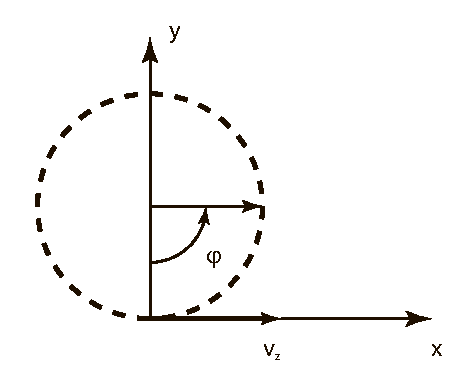
\includegraphics[width=0.5\textwidth]{images/im_02}
\end{wrapfigure}

Электрон совершает движение по окружности в плоскости \( xy \). 
В пространстве электрон перемещается по спирали.

Найдём координаты точки на экране. С учётом того \( v_{y0} = 0 \), уравнения 
движения перепишутся в виде:
\[
	\left\{ \begin{array}{ll}
		x = \cfrac{v\sin\alpha}{\omega_c}\sin\left( \omega_c t \right) \\
		y = -\cfrac{v\sin\alpha}{\omega_c}
			\Big[ 1 - \cos\left( \omega_c t \right) \Big]
	\end{array} \right.
\]

где \( t \) определяется выражением:
\(
	t = -\cfrac{mv_{z0}}{qE} + 
	\sqrt{ \cfrac{m}{qE}\left( \cfrac{mv^2\cos^2\alpha}{qE} + 2L \right)} 
\)

\pagebreak

%-------------------------------------------------------------------------------

\emph{Задача №2:} Сходящийся электронный поток эмитируется с торца 
цилиндрического катода радиуса \( R_k \), с начальной скоростью \( u \) и 
ускоряется под действием напряжения \( U_0 \) первого анода электронного 
прожектора, расположенного на расстоянии \( a \) от катода. Электроны вылетают 
под углами, определяемыми образующими конуса, вершины которого лежат на 
расстоянии \( 6a \) от катода. Первый анод представляет собой плоскость с 
круглой диафрагмой с радиусом \( R_0 = 2/3 R_k \). За этой плоскостью поток 
летит в продольном фокусирующем магнитном поле с величиной магнитной индукции 
\( B_0 \). Считая, что с катода снимается ток величиной \( I_k \), определить: 
период пульсации, максимальный радиус электронного потока и размер диафрагмы в 
первом аноде, при котором весь электронный поток проходит через диафрагму. 
Считать, что распределение поля между катодом и анодом и первым анодом 
эквивалентно распределению поля между двумя параллельными плоскостями.

\emph{Решение:}
\emph{Ответ:}

\end{document}
